\documentclass[aspectratio=169]{beamer}

\usetheme{Madrid}
\usecolortheme{default}
\usepackage{listings}
\usepackage{xcolor}
\usepackage{amsmath}
\usepackage{graphicx}
\usepackage{tikz}
\usetikzlibrary{shapes,arrows,positioning}

% Code styling
\lstset{
    language=Python,
    basicstyle=\ttfamily\small,
    keywordstyle=\color{blue},
    commentstyle=\color{gray},
    stringstyle=\color{orange},
    breaklines=true,
    showstringspaces=false,
    backgroundcolor=\color{lightgray!20}
}

\title{Sound Realty ML Model Serving}
\subtitle{Technical Architecture \& Implementation Deep Dive}
\author{ML Engineering Team}
\date{2026}

\begin{document}

\frame{\titlepage}

% ============= Slide 1: Executive Overview =============
\begin{frame}
\frametitle{Project Overview}
\begin{itemize}
    \item \textbf{Goal:} Deploy a KNN model for home price predictions
    \item \textbf{Input Data:} 18 property features + zipcode demographics
    \item \textbf{Model:} K-Nearest Neighbors (k=5) with RobustScaler normalization
    \item \textbf{Stack:} FastAPI, Python, scikit-learn, Docker
    \item \textbf{Architecture:} REST API with hot-reload model capability
    \item \textbf{Outcome:} Production-ready service with comprehensive testing \& monitoring
\end{itemize}
\end{frame}

% ============= Slide 1.5: Guidelines for Technical Deep Dive =============
\begin{frame}
\frametitle{Guidelines for developing the architecture and implementation}
\begin{itemize}
    \item \textbf{KISS:} Keep It Simple, Stupid - focus on core functionality. An MVP for a new client should prioritize reliability and maintainability over complex features.
    \item \textbf{Input Data:} make validation robust, but no need for complex feature engineering
    \item \textbf{Model:} Model improvement is a bonus, but focus on solid KNN implementation
    \item \textbf{Architecture:} keep it modular and easy to test locally
\end{itemize}
\end{frame}

% ============= Slide 2: BUILT ARCHITECTURE =============
\begin{frame}
\frametitle{Deployed Architecture Overview}

\begin{center}
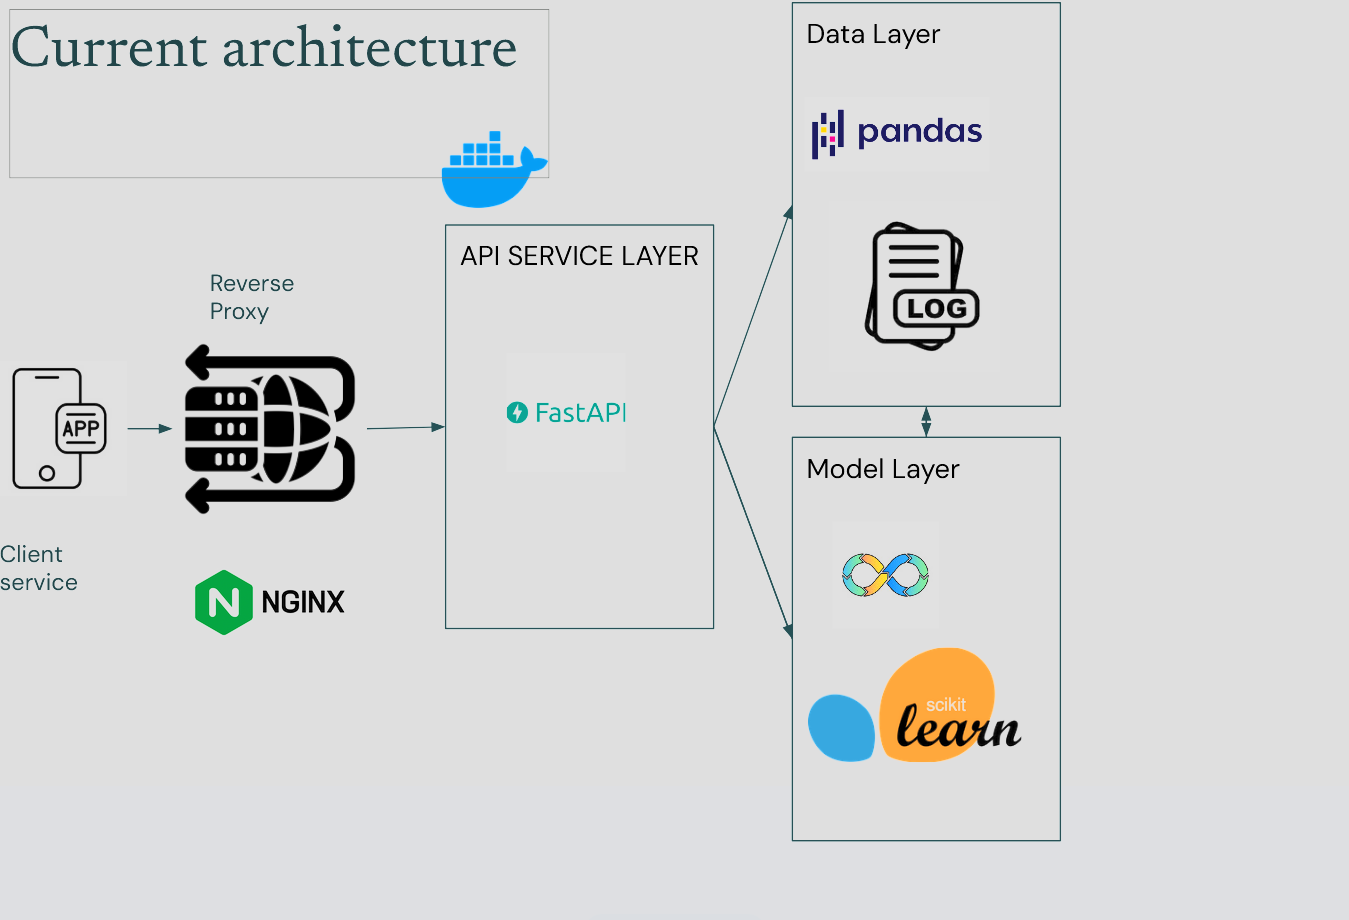
\includegraphics[width=0.6\textwidth]{../images/current_architecture.png}
\end{center}

\end{frame}

\begin{frame}
\frametitle{Scaling Architecture Overview}

\begin{center}
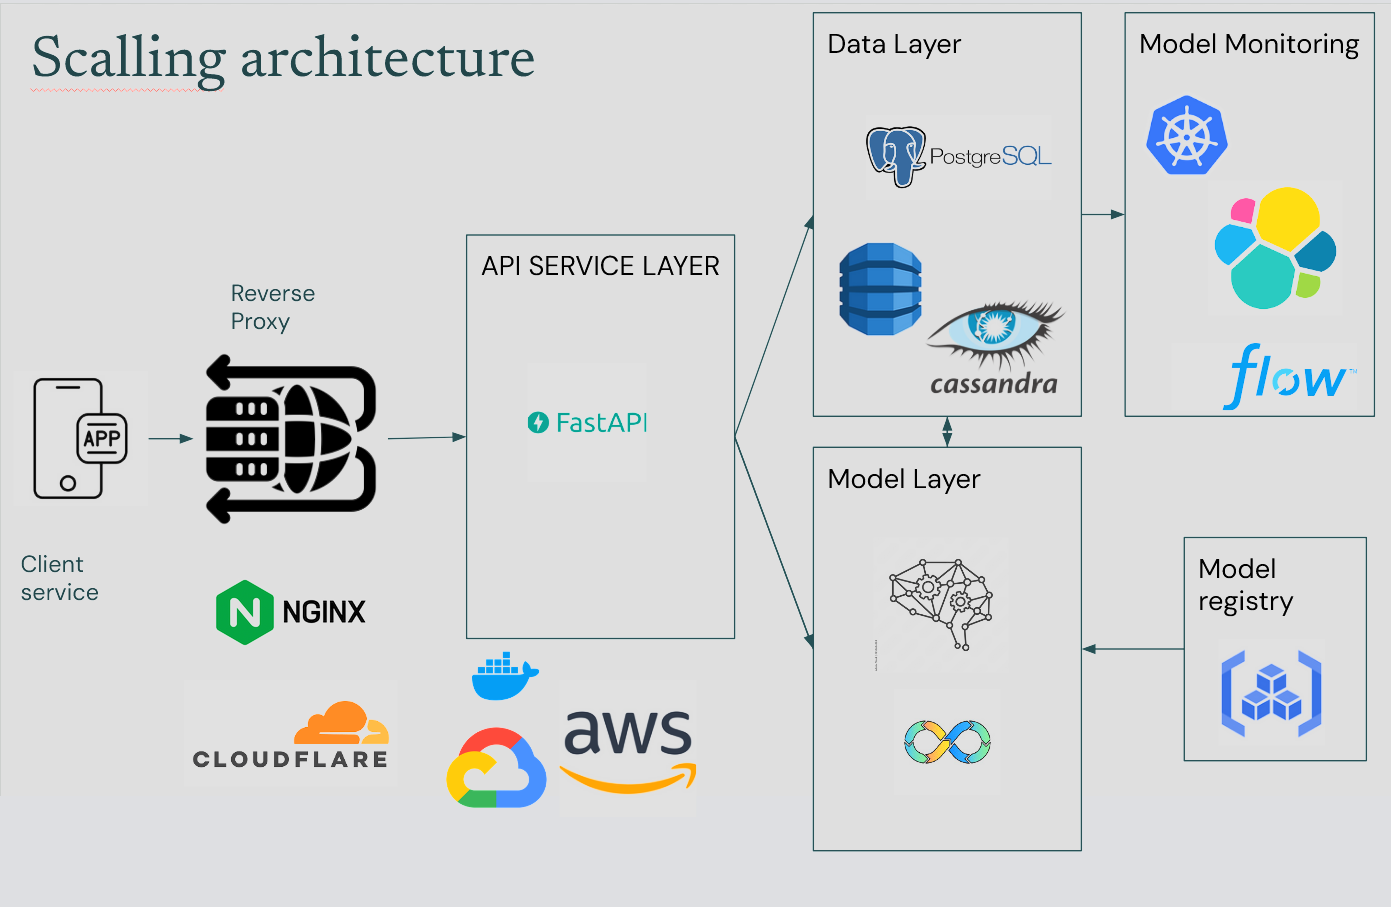
\includegraphics[width=0.6\textwidth]{../images/scalling_architecture.png}
\end{center}

\end{frame}


% ============= Slide 3: Data Pipeline =============
\begin{frame}[fragile]
\frametitle{Data Pipeline \& Feature Engineering}

\textbf{Data Sources:}
\begin{itemize}
    \item KC House Sales (21,613 records)
    \item Zipcode Demographics
    \item Feature-engineered variants
\end{itemize}

\textbf{Feature Set:} Primary (bedrooms, bathrooms, sqft\_living, grade), Secondary (lat/long, year\_built), Demographic (population, income, education)

\vspace{0.3cm}
\textbf{Data Integration:}
\begin{lstlisting}[basicstyle=\ttfamily\tiny]
# Merge demographics by zipcode
merged = sales.merge(demographics, how='left', on='zipcode')
\end{lstlisting}

\textbf{Preprocessing:} RobustScaler (handles outliers), 80-20 train-test split, Feature importance analysis
\end{frame}

% ============= Slide 4: Model Selection =============
\begin{frame}
\frametitle{Model Architecture: KNN Regression}

\textbf{Why KNN?}
\begin{itemize}
    \item \textbf{Interpretability:} Predictions based on $k$ nearest training samples
    \item \textbf{Non-parametric:} Captures complex non-linear relationships
    \item \textbf{No training phase:} Instantaneous retraining possible
    \item \textbf{Baseline:} okay performance on housing datasets
\end{itemize}

\vspace{0.3cm}
\textbf{Model Pipeline:}
\[
\text{RawFeatures} \xrightarrow{\text{RobustScaler}} \text{NormalizedFeatures} \xrightarrow{\text{KNN (k=5)}} \text{Price Prediction}
\]

\vspace{0.3cm}
\textbf{Performance Metrics:}
\begin{itemize}
    \item Test RMSE: \$175K-\$185K (varies by feature set)
    \item Test MAE: \$105K-\$115K
    \item Test R² Score: 0.82-0.84
    \item MAPE: 22-24\%
\end{itemize}
\end{frame}

% ============= Slide 5: Model Variants =============
\begin{frame}[fragile]
\frametitle{Model Versioning \& A/B Testing}

\textbf{Multiple Model Variants:}
\begin{itemize}
    \item \textbf{Basic Model:} 10 numeric features only
    \item \textbf{Added Features Model:} 18 features + demographics
    \item \textbf{Future Variants:} Gradient Boosting, Neural Networks
\end{itemize}

\vspace{0.3cm}
\textbf{Model Storage Structure:}
\begin{lstlisting}
model/
  ├── basic/
  │   ├── model.pkl (KNN pipeline)
  │   ├── model_features.json
  │   └── metrics.json
  ├── added_features/
  │   ├── model.pkl
  │   └── model_features.json
  └── 2026-03-05_05/ (timestamp-based)
\end{lstlisting}

\textbf{Hot-Reload Capability:} Switch models via environment variable without API restart
\end{frame}

% ============= Slide 6: API Architecture =============
\begin{frame}[fragile]
\frametitle{API Design: REST Endpoints}

\textbf{Endpoint \#1: Health Check}
\begin{lstlisting}
GET /health → {status: 'healthy', models_loaded: true}
\end{lstlisting}

\textbf{Endpoint \#2: Full Prediction (18 fields)}
\begin{lstlisting}
POST /predict
{
  bedrooms, bathrooms, sqft_living, grade, ..., zipcode
}
→ {prediction: $850K, model_version: 'added_features'}
\end{lstlisting}

\textbf{Endpoint \#3: Minimal Prediction (8 fields)}
\begin{lstlisting}
POST /predict-minimal (uses basic model)
\end{lstlisting}

\textbf{API Framework: FastAPI}
\begin{itemize}
    \item Async/await for concurrent request handling
    \item Pydantic validation with automatic OpenAPI docs
    \item Lifespan context manager for startup/shutdown
\end{itemize}
\end{frame}

% ============= Slide 7: Production Monitoring =============
\begin{frame}[fragile]
\frametitle{Monitoring \& Observability}

\textbf{Model Call Logging:}
\begin{itemize}
    \item Every prediction logged with timestamp, input features, output
    \item Client metadata: IP, user-agent, endpoint
    \item Latency tracking for performance monitoring
    \item Structured JSON format for analysis
\end{itemize}

\vspace{0.3cm}
\textbf{What We Track:}
\begin{lstlisting}
{
  "timestamp": "2026-03-05T10:23:45Z",
  "model_version": "added_features",
  "input_features": {...},
  "prediction": 850000,
  "latency_ms": 12.5,
  "client_ip": "192.168.1.1"
}
\end{lstlisting}

\textbf{Benefits:}
\begin{itemize}
    \item Model drift detection (compare recent vs. baseline predictions)
    \item Data quality monitoring (detect invalid inputs)
    \item Usage analytics \& feature analysis
\end{itemize}
\end{frame}

% ============= Slide 8: Quality Assurance =============
\begin{frame}
\frametitle{Testing Strategy}

\textbf{Test Coverage (pytest):}
\begin{itemize}
    \item \textbf{API Tests:} Endpoint validation, edge cases, error handling
    \item \textbf{Model Tests:} Prediction outputs, model switching, feature loading
    \item \textbf{Integration Tests:} Full pipeline (data → prediction)
    \item \textbf{Logger Tests:} Call logging, JSON serialization
\end{itemize}

\vspace{0.3cm}
\textbf{Key Test Scenarios:}
\begin{itemize}
    \item Invalid input handling (missing fields, type mismatches)
    \item Model hot-reload (switching between versions)
    \item Prediction consistency (deterministic output)
    \item Data processing (demographics merge, feature ordering)
\end{itemize}

\vspace{0.3cm}
\textbf{CI/CD:} pytest automatically runs on every commit
\end{frame}

% ============= Slide 9: Deployment =============
\begin{frame}[fragile]
\frametitle{Containerization \& Deployment}

\textbf{Docker Strategy:}
\begin{lstlisting}
FROM python:3.10-slim
COPY requirements.txt .
RUN pip install -r requirements.txt
COPY . .
CMD ["uvicorn", "src.api.main:app", "--host", "0.0.0.0"]
\end{lstlisting}

\textbf{Docker Compose Orchestration:}
\begin{itemize}
    \item FastAPI service on port 8000
    \item Nginx reverse proxy on port 80
    \item Volume mounts for model persistence
    \item Environment-based model selection
\end{itemize}

\vspace{0.3cm}
\textbf{Production Considerations:}
\begin{itemize}
    \item Stateless design for horizontal scaling
    \item Lazy loading to minimize startup time
    \item Graceful shutdown with lifespan context
\end{itemize}
\end{frame}

% ============= Slide 10: Performance Analysis =============
\begin{frame}
\frametitle{Performance Insights}

\textbf{Model Performance (Test Set):}
\begin{table}
\begin{tabular}{|l|c|c|c|}
\hline
\textbf{Metric} & \textbf{Basic} & \textbf{Added Features} & \textbf{Unit} \\
\hline
RMSE & 180K & 175K & \$ \\
\hline
MAE & 110K & 105K & \$ \\
\hline
R² Score & 0.82 & 0.84 & - \\
\hline
MAPE & 23\% & 22\% & \% \\
\hline
\end{tabular}
\end{table}

\vspace{0.3cm}
\textbf{Bias Analysis:}
\begin{itemize}
    \item Underpricing occurs ~18\% of the time (bad for sellers)
    \item Weighted RMSE penalizes underprediction 2x
    \item Feature importance: sqft\_living \& grade dominate
\end{itemize}

\vspace{0.3cm}
\textbf{Inference Latency:} \textbf{8-15ms} per prediction (GPU not required)
\end{frame}

% ============= Slide 11: Key Engineering Decisions =============
\begin{frame}
\frametitle{Engineering Decisions \& Trade-offs}

\textbf{Decision 1: KNN over Gradient Boosting}
\begin{itemize}
    \item \textbf{Pro:} Hot-reload capability, interpretability, fast inference
    \item \textbf{Con:} Slower than GB for very large feature spaces; memory-dependent
\end{itemize}

\vspace{0.3cm}
\textbf{Decision 2: RobustScaler over StandardScaler}
\begin{itemize}
    \item \textbf{Reasoning:} Housing prices have outliers; RobustScaler is median-based
\end{itemize}

\vspace{0.3cm}
\textbf{Decision 3: Lazy Loading of Models}
\begin{itemize}
    \item \textbf{Pro:} Fast startup, multiple models in memory
    \item \textbf{Con:} First request slightly slower
\end{itemize}

\vspace{0.3cm}
\textbf{Decision 4: Structured Logging}
\begin{itemize}
    \item JSON logs enable machine-readable analysis, drift detection
\end{itemize}
\end{frame}

% ============= Slide 13: Production Metrics =============
\begin{frame}
\frametitle{Production Monitoring Dashboard}

\textbf{Key Metrics to Track:}
\begin{itemize}
    \item \textbf{Throughput:} Requests/second
    \item \textbf{Latency:} P50, P95, P99 latencies
    \item \textbf{Model Drift:} Mean absolute error of recent predictions vs. baseline
    \item \textbf{Data Quality:} \% of invalid inputs caught by validation
    \item \textbf{Prediction Distribution:} Are we making reasonable price estimates?
\end{itemize}

\vspace{0.3cm}
\textbf{Alerting Thresholds:}
\begin{itemize}
    \item API latency > 100ms
    \item Error rate > 1\%
    \item Prediction mean shifts > 5\% from baseline
    \item Memory usage > 80\%
\end{itemize}

\vspace{0.3cm}
\textbf{Retraining Trigger:} Model drift detected (weekly comparison) or RMSE degrades
\end{frame}

% ============= Slide 15: Technical Q&A =============
\begin{frame}[fragile]
\frametitle{Questions for Technical Discussion}

\textbf{Potential Discussion Topics:}
\begin{enumerate}
    \item Why not use dimensionality reduction (PCA) given 18 features?
    \item How would you handle categorical features (e.g., zipcode as categorical)?
    \item What's your strategy for handling missing demographics data?
    \item How do you prevent data leakage in train-test split?
    \item What about outlier detection before prediction?
    \item How would you implement online learning / continual retraining?
    \item Prediction intervals vs. point estimates?
\end{enumerate}

\end{frame}

\end{document}
